\documentclass{article}
\usepackage[french]{babel}
\usepackage[T1]{fontenc}
\usepackage[utf8]{inputenc}
\usepackage{graphicx} % Required for inserting images
\usepackage{listingsutf8}
\lstset{%
    inputencoding=utf8,
    literate=
        {é}{{\'e}}{1}%
        {è}{{\`e}}{1}%
        {à}{{\`a}}{1}%
        {â}{{\^a}}{1}%
        {ç}{{\c{c}}}{1}%
        {œ}{{\oe}}{1}%
        {ù}{{\`u}}{1}%
        {É}{{\'E}}{1}%
        {È}{{\`E}}{1}%
        {À}{{\`A}}{1}%
        {Ç}{{\c{C}}}{1}%
        {Œ}{{\OE}}{1}%
        {Ê}{{\^E}}{1}%
        {ê}{{\^e}}{1}%
        {î}{{\^i}}{1}%
        {ï}{{\"i}}{1}%
        {ô}{{\^o}}{1}%
        {û}{{\^u}}{1}%
}
\usepackage{fullpage}
\usepackage{setspace}
\usepackage{todonotes}
\usepackage{amsthm}
\usepackage{amsmath}
\usepackage{amssymb}
\usepackage[all]{xy}

\usepackage[french, frenchkw, boxed, linesnumbered]{algorithm2e}

\newtheoremstyle{exostyle}% style name
{10pt}% above space
{10pt}% below space
{}% body font
{}% indent amount
{\scshape\bfseries\large}% head font
{\hfill\vspace{5pt}\newline}% post head punctuation
{0pt}% Space after theorem head
{\hfill\thmname{#1}\thmnumber{ #2} -- \thmnote{ #3}}% head spec

\newtheoremstyle{partiestyle}% style name
{1em}% above space
{1em}% below space
{}% body font
{}% indent amount
{\bfseries}% head font
{\vspace{.5em}\newline}% post head punctuation
{0em}% Space after theorem head
{\thmnumber{#2} \thmnote{ #3}}% head spec

\newtheoremstyle{questionstyle}% style name
{.5em}% above space
{.5em}% below space
{}% body font
{}% indent amount
{\bfseries}% head font
{}% post head punctuation
{0em}% Space after theorem head
{Question \thmnumber{#2 }}% head spec

\theoremstyle{exostyle}
\newtheorem{exo}{Exercice}

\theoremstyle{partiestyle}
\newtheorem{partie}{}[exo]

\theoremstyle{questionstyle}
\newtheorem{question}{Question}[exo]
\newtheorem{questionpartie}{Question}[partie]

\title{Devoir Surveillé Algorithmie Avancée}
\author{L3 MPCI}
\date{11 octobre 2024 - Durée: 2h}

\begin{document}

\maketitle

\begin{center}
{\em\bf Lorsque l'on vous demande d'écrire de décrire ou de donner un algorithme cela signifiera toujours en donner un pseudo-code, justifier de son exactitude et de sa complexité}

~\\

{\em On rappelle qu'aucun document ni équipement électrique ou électronique n'est autorisé. }
\end{center}


\paragraph*{Les exercices :}
\begin{itemize}
\item sont au nombre de 4;
\item sont indépendants;
\item ont un début plus facile que la fin.
\end{itemize}

\clearpage

\begin{exo}[Débit de réseau]

	Dans un réseau de communication, on appelle {\it débit} la quantité d'information que le réseau garantit de pouvoir faire passer entre deux sommets. Dans cet exercice, le réseau est modélisé par un graphe $G = (X, E)$ connexe. Chaque arête est munie d'une bande passante (qui ici sera appelée poids), $v: E\to \mathbb{R}^+$, qui limite la quantité d'information qu'elle peut véhiculer. Le but de l'exercice est de mettre au point des algorithmes permettant de calculer le
débit. Le graphe de la figure~\ref{fig-transport} va servir d'exemple.
	\begin{figure}[h!]
	\begin{center}
	$$
	\xy
	\xymatrix{
	I_6 \ar@{-}[rr]^2  
	    \ar@{-}[drr]^3
	    \ar@{-}[ddrr]^1 
	    \ar@{-}[ddd]^1&& I_1 &&
	I_2 \ar@{-}[ll]_5  
	    \ar@{-}[dll]_6
	    \ar@{-}[ddll]_3 
	    \ar@{-}[ddd]^6 \\
	&&I_5\ar@{-}[u]^{14}  
	    \ar@{-}[d]^{11}
	&&\\
	&&I_4&&\\
	I_8 \ar@{-}[rrrr]^8  
	    \ar@{-}[urr]_{15}
	    \ar@{-}[uurr]_{12} 
	    \ar@{-}[uuurr]^{11}
	&&&&I_9\ar@{-}[ull]^9  
	    \ar@{-}[uuull]^4}
	\endxy
	$$
	\end{center}
	\caption{Un réseau de transport\label{fig-transport}}
\end{figure}


\begin{partie}
	\begin{questionpartie}
		Montrer que si $\mathcal{C}_{xy}$ est l'ensemble des chemins entre $x$ et $y$ alors le débit entre $x$ et $y$ s'écrit :
			$$
			D(x, y) = \max(\{ \min(\{v(x_ix_{i+1}) \vert 0 \leq i < k\}) \vert x_0 \dots x_k \in  \mathcal{C}_{xy} \})
			$$
	\end{questionpartie}
		
\begin{questionpartie}
En déduire, à l'aide d'arguments simples, que la chaîne de débit maximum entre $I_6$ et $I_2$ pour le graphe exemple a un débit
égal à trois.
\end{questionpartie}
\end{partie}	
\begin{partie}
Soit $T$ un arbre couvrant de $G$ de poids maximum (le
poids de $T$ étant la somme, sur toutes les arêtes de $T$, des poids
de ces arêtes). On appelle $T_1$ et $T_2$ les deux composantes que
l'on obtient, à partir de $T$, en enlevant l'arête de poids minimum
sur la chaîne de $T$ entre $x$ et $y$. Prouver que la valuation minimale de la chaîne de $T$
joignant $x$ et $y$ vaut $D(x, y)$ pour le réseau $G$.

\end{partie}	

\begin{partie}
Donner un algorithme déterminant, dans un arbre
quelconque, l'unique chaîne entre deux sommets donnés.
\end{partie}	

\begin{partie}
Quelle méthode peut-on appliquer pour déterminer, dans
un graphe quelconque $G$, une chaîne de débit maximum entre deux
sommets quelconques de $G$ ?
\end{partie}	

\begin{partie}
	Appliquer cette méthode pour déterminer une chaîne de
	débit maximum entre $I_1$ et $I_4$ dans le réseau exemple.
\end{partie}	

\end{exo}

\begin{exo}[Réduction]
On considère le problème suivant :

\begin{itemize}
	\item {\bf nom :} Couverture
	\item {\bf entrée :} un graphe $G=(V, E)$ et un entier $k$
	\item {\bf question :} existe-t-il $V' \subseteq V$ avec $\vert V' \vert \leq k$ tel que toute arête de $G$ possède au moins une extrémité dans $V'$ ?
\end{itemize}

\begin{partie}
	Donner une couverture de cardinal minimum (justifier le) pour le graphe de la figure~\ref{degres}.
\end{partie}	

\begin{partie}
	Montrez que le problème couverture est dans NP.
\end{partie}
\begin{partie}
		Montrez que le problème couverture est NP-complet (toutes les reductions du cours sont utilisables).
\end{partie}
	
\end{exo}

\begin{exo}[Degrés des somments d'un graphe]
	Le but de cet exercice est de donner des pistes pour déterminer si une suite de $n$ entiers peut être vue comme les degrés d'un graphe à $n$ sommets. Par exemple la suite $(1, 2, 2, 3, 3, 3, 4)$ admet le graphe de la figure~\ref{degres} :
	
	\begin{figure}[h!]
		\begin{center}
			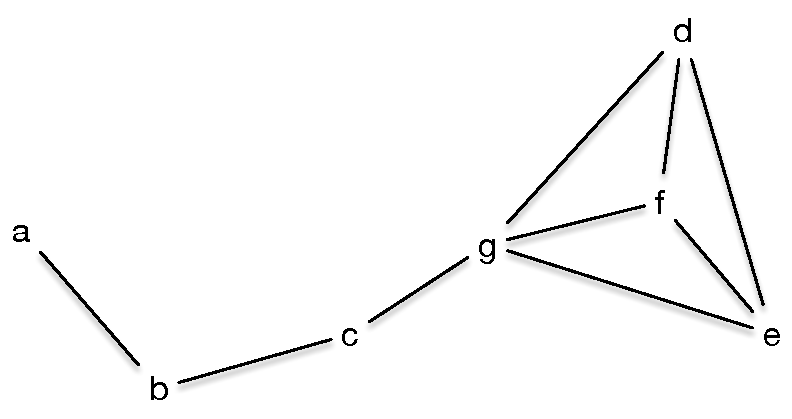
\includegraphics[scale=.35]{degrés-1.pdf}
		\end{center}
		\caption{Les sommets $(a,b, c, d, e, f, g)$ ont respectivement pour degré $(1, 2, 2, 3, 3, 3, 4)$\label{degres}}
	\end{figure}
\begin{partie}
Montrer que la somme des entiers est nécessairement paire pour qu'un tel graphe existe, mais que cette condition n'est pas suffisante.
\end{partie}

\begin{partie}
	Nous allons ici résoudre ce problème pour les graphes orientés grâce à la théorie des flots. Soit $n$ un entier positif. On considère $2n$ entiers positifs ou nuls, notés $d^+_1, \dots d^+_i, \dots d^+_n$ et $d^-_1, \dots d^-_i, \dots d^-_n$. On cherche à construire un graphe {\bf orienté} $G = (V, E)$ sans boucle ni d’arc multiple dont les sommets, notés $x_1, \dots, x_i\dots , x_n$, vérifient $\delta^+(x_i) = d^+_i$ et $\delta^-(x_i) = d^-_i$ pour $1\leq i \leq n$,
	\begin{questionpartie}
		Modéliser le problème sous forme d’un problème de flot maximum. Exprimer à l’aide de n la complexité de l’algorithme de Ford et Fulkerson quand on l’applique à ce problème.
	\end{questionpartie}
	Résoudre le problème pour $n=5$ et
		\begin{itemize}
			\item $d^+_1 = 2$, $d^+_2 = 3$, $d^+_3 = 1$, $d^+_4 = 1$, $d^+_5 = 3$,
			\item $d^-_1 = 2$, $d^-_2 = 1$, $d^-_3 = 2$, $d^-_4 = 2$, $d^-_5 = 3$,
		\end{itemize}	
	\begin{questionpartie}
		Est-il possible d'adapter le modèle pour des graphes non dirigé ? Si oui, montrez la construction pour le graphe de la figure~\ref{degres}. 
	\end{questionpartie}
\end{partie}
\begin{partie}	
	Vous aller caractériser les graphes à $n>k$ sommets tels que $\delta(x) = k$ pour tout sommet $x$. Ces graphes sont appelés $k$-régulier.
	\begin{questionpartie}
		Montrer qu'il est nécessaire que $k\cdot n$ soit pair pour qu'un graphe $k$-régulier existe.
	\end{questionpartie}
	\begin{questionpartie}
		Montrez que si $n=2m$ et $m\geq k$ on peut construire un graphe biparti $k$-régulier.
	\end{questionpartie}
	\begin{questionpartie}
		Montrez que si $k=2m$ on peut construire un graphe $k$-régulier pour tout $n\geq k+1$.
	\end{questionpartie}
	\begin{questionpartie}
		Montrer qu'il est suffisant que $k\cdot n$ soit pair pour qu'un graphe $k$-régulier existe.
	\end{questionpartie}
	
\end{partie}
\end{exo}

\begin{exo}[Chemins dans un cylindre]
On considère le problème suivant :
On considère $n\cdot p$ entiers positifs $a_{ij}$ ($1\leq i\leq n, 1\leq
j\leq p$), écrits sur un cylindre ayant $n$ lignes et $p$ colonnes,
comme illustré figure~\ref{cyl1}.

\begin{figure}[h!]
\begin{center}
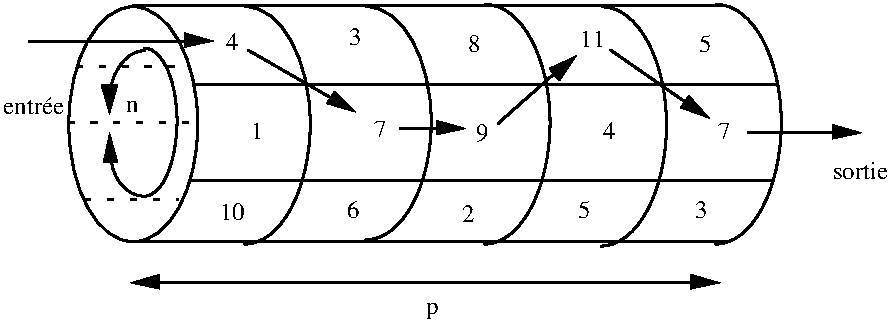
\includegraphics[scale=0.45]{Cyl1.pdf}
\caption{Le cylindre\label{cyl1}} 
\end{center}
\end{figure}

Un chemin est tracé de l'entrée du cylindre jusqu'à la sortie, avec la
restriction que, d'une case, on ne peut aller qu'aux trois positions
de la colonne suivante adjacentes à la position courante. Le coût d'un
tel chemin est la somme des entiers écrits dans les cases traversées
(par exemple, le chemin tracé sur le dessin a un coût égal à 38).

\begin{partie}
Combien de chemins distincts a-t-on de l'entrée à la
sortie, sans imposer les cases de départ et d'arrivée ?
\end{partie}
\begin{partie}
Expliciter un algorithme, prenant en entrée tous les $a_{ij}$ ($1\leq i\leq n, 1\leq
j\leq p$), qui détermine un tel chemin de
coût minimum en $\mathcal{O}(np)$ opérations. On justifiera le fait
que l'algorithme calcule bien ce qu'il faut, ainsi que sa complexité.
\end{partie}
\begin{partie}
L'appliquer à l'exemple de la figure~\ref{cyl2} où le cylindre
a été déplié ($n=4, p=5$~; les bords $ab$ et $cd$ sont confondus), et
en déduire un chemin de coût minimum.

\begin{figure}[h!]
\begin{center}
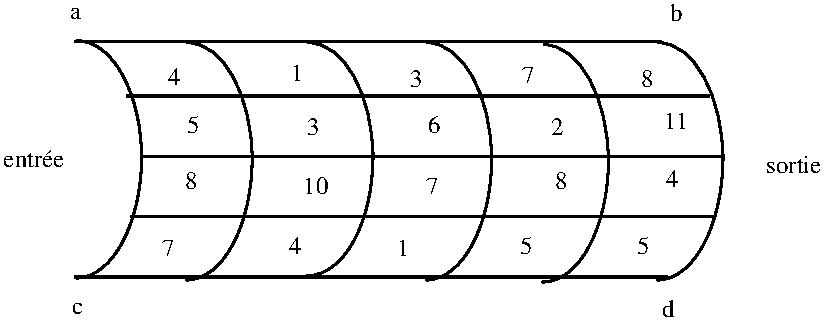
\includegraphics[scale=0.45]{Cyl2.pdf}
\caption{Le cylindre (après aplatissement)\label{cyl2}}
\end{center}
\end{figure}
\end{partie}
	
\begin{partie}
A l'aide de l'algorithme de Dijkstra, retrouver le
chemin précédent. Du point de vue de la complexité, lequel des deux
algorithmes est-il le plus avantageux d'appliquer pour résoudre ce
problème ?
\end{partie}

\end{exo}

\end{document}
